\documentclass{article}
\usepackage[utf8]{inputenc}
\usepackage{hyperref}
\usepackage{graphicx}
\usepackage[a4paper, left = 3cm, right = 3cm, top =2cm]{geometry}
\title{\textbf{\underline{Proyecto de Matemática Numérica}} \\ \textit{Predicción de crecimiento demográfico.} \\ \textit{Informe \#2}}
\author{Luis Ernesto Serras Rimada \\ Guillermo Cepero García \\ Miguel Vadim Vilariño Pedraza}

\date{\today}
\begin{document}
\maketitle
    Informe Plantilla
    \tableofcontents
    Introduccion
\newpage
\section{Desarrollo}
Desarrollo\\
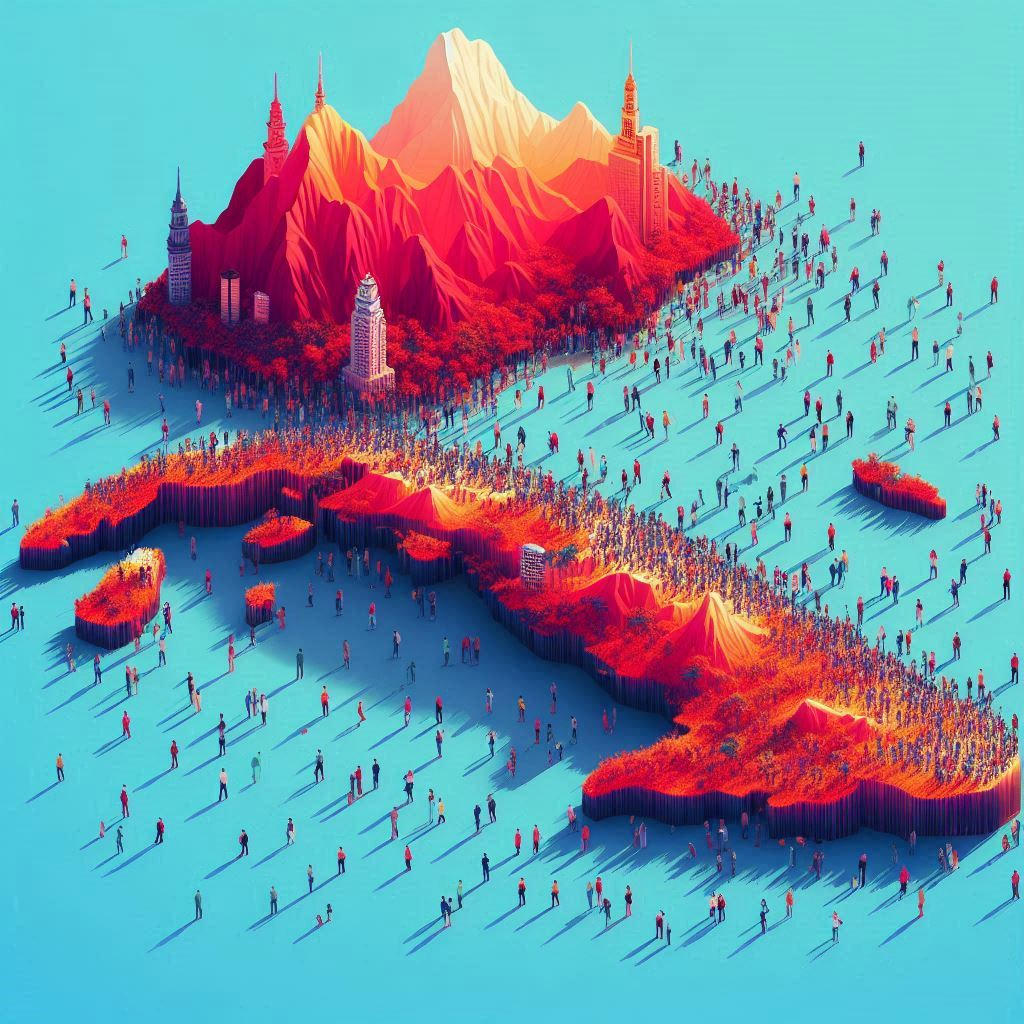
\includegraphics[height = 7cm]{img/cuba3.jpeg}

\newpage
\subsection{subsection}
\clearpage

\section{Conclusiones}

\cleardoublepage
\section{Referencias}
\url{https://github.com/LFrench03/Modelo-de-Crecimiento-Poblacional/blob/main/data/csv/poblacion-residente.csv}
\\\textit{\textbf{\underline{Referencias}}:}
\begin{itemize}
    \item (1)
\end{itemize}

\end{document}